\documentclass[11pt]{article}

\usepackage[a4paper,margin=1in]{geometry}
\usepackage[utf8]{inputenc}
\usepackage[T1]{fontenc}
\usepackage{amsmath,amsfonts,amssymb}
\usepackage{graphicx}
\usepackage{booktabs}
\usepackage{multirow}
\usepackage{algorithm}
\usepackage{algorithmic}
\usepackage{caption}
\usepackage{subcaption}
\usepackage{hyperref}
\usepackage{cite}
\usepackage{pgfplots}
\pgfplotsset{compat=1.18}

\title{An Adaptive Latent Semantic Analysis Framework for Binary Text Classification}

\author{Touza Isaac\\
	Department of Mathematics and Computer Science, Faculty of Science\\
	University of Maroua, Cameroon\\
	\texttt{isaac.touza@univ-maroua.cm}}
\date{}

\begin{document}
	\maketitle

	\begin{abstract}
		Binary text classification is a fundamental task in natural language processing, typically addressed using discriminative machine learning models or deep neural architectures. While Latent Semantic Analysis (LSA) has historically played an important role in semantic representation, it is now largely confined to a preprocessing function due to its static and task-independent formulation. This paper proposes an \textit{Adaptive Latent Semantic Analysis (A-LSA)} framework that redefines LSA as a discriminative, class-aware classification model. The proposed approach constructs class-conditional latent semantic spaces and introduces a semantic differential distance as a direct decision criterion. Experimental results on three benchmark datasets demonstrate that A-LSA achieves strong performance on short texts (F1=0.95 on SMS Spam, only 1.6\% below state-of-the-art) where class semantics are highly discriminative, while revealing limitations on longer, more complex documents. The approach maintains superior interpretability through explicit semantic axes and achieves computational efficiency suitable for real-time applications. These results establish clear applicability boundaries for class-conditional semantic models and demonstrate that A-LSA offers a valuable alternative for applications requiring transparency, efficiency, and working with short, semantically-distinct text categories.
	\end{abstract}

	\textbf{Keywords}: Binary classification, Latent semantic analysis, Semantic distance, Interpretable NLP, Low-resource AI, Supervised learning

	%---------------------------------------------------

	\section{Introduction}

	Binary text classification constitutes a cornerstone of numerous natural language processing (NLP) applications, including spam filtering, sentiment analysis, topic detection, and decision support systems~\cite{sebastiani2002,aggarwal2012}. Deep learning models, particularly transformer-based architectures such as BERT~\cite{devlin2019} and its variants, currently dominate this field due to their remarkable empirical performance. However, these models suffer from several significant limitations: high computational cost (millions of parameters requiring substantial GPU resources), lack of transparency in the decision-making process, and critical dependence on large annotated datasets~\cite{lipton2018,rudin2019}.

	In contexts where computational resources are limited, interpretability is crucial, or annotated data is scarce---situations frequently encountered in developing countries or specialized domains---these models become difficult to apply. There is therefore a pressing need for alternative methods offering a balance between performance, efficiency, and transparency.

	Latent Semantic Analysis (LSA), initially proposed by Deerwester et al.~\cite{deerwester1990}, provides a mathematically grounded framework for discovering latent semantic structures through matrix factorization via Singular Value Decomposition (SVD). Despite its mathematical elegance, intrinsic interpretability, and computational efficiency, LSA is typically relegated to a role as a static dimensionality reduction technique, followed by an external classifier such as logistic regression or support vector machine~\cite{sebastiani2002,landauer1997}. This approach ignores a fundamental aspect: the semantic asymmetry between classes in supervised classification tasks.

	This paper challenges this established paradigm by introducing \textit{Adaptive Latent Semantic Analysis (A-LSA)}, which directly integrates class information into the latent space construction process, thereby transforming LSA from an unsupervised dimensionality reduction tool into a discriminative semantic classifier in its own right.

	The main contributions of this work are as follows:
	\begin{itemize}
		\item A class-conditional formulation of LSA for binary classification, enabling the capture of distinct semantic specificities of each class through separate latent spaces.
		\item A semantic differential distance as a direct decision function, offering an intuitive and geometrically motivated interpretation of predictions.
		\item A data-driven threshold adjustment mechanism based on weighted mean differential distances, providing robust adaptation to class imbalance without requiring prior-based heuristics.
		\item A theoretical analysis of the connection between minimizing conditional reconstruction error and maximizing inter-class separability.
		\item A comprehensive experimental evaluation on three benchmark datasets with varying text lengths and semantic characteristics, revealing clear performance boundaries: strong results on short texts (F1=0.946 on SMS Spam, only 1.6\% below state-of-the-art) and substantial performance degradation on longer, complex documents (F1=0.705-0.780 on IMDb and 20 Newsgroups).
		\item A detailed sensitivity analysis on the impact of latent dimension \( k \) and class imbalance, along with geometric visualization of latent space separability using t-SNE.
		\item An empirical demonstration that explained variance ratio serves as a reliable predictor of A-LSA's effectiveness, establishing quantitative criteria (>30\% per class) for model applicability.
	\end{itemize}

	The remainder of the paper is organized as follows: Section~\ref{sec:related} presents related work, Section~\ref{sec:problem} formalizes the problem, Section~\ref{sec:method} details the proposed A-LSA method, Section~\ref{sec:experiments} presents experimental results, and Section~\ref{sec:conclusion} concludes with future perspectives.

	%---------------------------------------------------

	\section{Related Work}
	\label{sec:related}

	\subsection{Latent semantic analysis and its extensions}

	Latent Semantic Analysis (LSA) has been widely used in information retrieval and semantic similarity tasks since its initial proposal~\cite{deerwester1990,landauer1997}. LSA is based on the hypothesis that words appearing in similar contexts have similar meanings, and uses SVD to extract a reduced-dimension representation capturing this latent structure.

	Probabilistic extensions have been proposed to address certain statistical limitations of LSA. Probabilistic Latent Semantic Analysis (PLSA)~\cite{hofmann1999} introduces a probabilistic generative model based on non-negative matrix decomposition. Latent Dirichlet Allocation (LDA)~\cite{blei2003} generalizes this approach by adding Dirichlet priors, enabling better generalization. However, these methods remain fundamentally unsupervised and do not leverage the class labels available in supervised classification tasks.

	\subsection{Supervised text classification}

	In supervised classification pipelines, LSA is commonly combined with discriminative classifiers such as Support Vector Machines (SVM), Logistic Regression, or Neural Networks~\cite{sebastiani2002,aggarwal2012}. While effective, this two-stage strategy treats LSA as a generic preprocessing step, ignoring the semantic asymmetry between classes. Building a single latent space for all classes may dilute discriminative features specific to each class.

	Modern text classification methods primarily rely on pre-trained word embeddings (Word2Vec~\cite{mikolov2013}, GloVe~\cite{pennington2014}) or contextual language models based on transformers (BERT~\cite{devlin2019}, RoBERTa~\cite{liu2019}). These approaches have revolutionized NLP by achieving state-of-the-art performance on numerous tasks. Recent hybrid approaches, such as SHADO~\cite{touza2025}, combine semantic representations with domain ontologies to improve classification while preserving interpretability. However, the computational complexity, dependence on large amounts of training data, and decision-making opacity of deep learning models limit their applicability in certain contexts.

	\subsection{Interpretability and responsible AI}

	Recent research emphasizes the critical importance of interpretability in AI systems, particularly for high-stakes applications (medicine, justice, finance)~\cite{rudin2019,molnar2020}. Rudin~\cite{rudin2019} argues convincingly that it is preferable to use inherently interpretable models rather than attempting to explain black-box models post-hoc. Post-hoc explanation methods (LIME~\cite{ribeiro2016}, SHAP~\cite{lundberg2017}) can be misleading and do not guarantee faithful understanding of the decision-making process.

	\subsection{Positioning of our contribution}

	Our work distinguishes itself from existing approaches by revisiting a classic semantic model (LSA) from a resolutely discriminative and supervised perspective. Unlike two-stage pipelines and hybrid frameworks such as SHADO~\cite{touza2025}, A-LSA integrates supervision directly into the construction of the latent semantic space, creating class-specific representations without requiring external knowledge structures. This approach fills an important gap in the literature by demonstrating that it is possible to achieve competitive performance with much more complex models while preserving interpretability and computational efficiency.

	%---------------------------------------------------

	\section{Problem Formulation}
	\label{sec:problem}

	\subsection{Definitions and notation}

	Let \( D = \{(d_i, y_i)\}_{i=1}^{N} \) be a labeled corpus, where \( d_i \) represents the i-th text document and \( y_i \in \{0,1\} \) its binary class label. Each document is represented by a TF-IDF vector \( \mathbf{x}_i \in \mathbb{R}^{m} \), where \( m \) denotes the vocabulary size. The global term-document matrix is denoted \( \mathbf{X} \in \mathbb{R}^{m \times N} \), whose column \( i \) corresponds to vector \( \mathbf{x}_i \).

	The TF-IDF (Term Frequency-Inverse Document Frequency) weighting for a term \( t \) in a document \( d \) is defined as:
	\begin{equation}
		\text{TF-IDF}(t,d) = \text{TF}(t,d) \times \log\left(\frac{N}{\text{DF}(t)}\right)
	\end{equation}
	where \( \text{TF}(t,d) \) is the frequency of term \( t \) in document \( d \), and \( \text{DF}(t) \) is the number of documents containing term \( t \).

	\subsection{Classical LSA: formulation and limitations}

	Classical LSA constructs a global term-document matrix \( \mathbf{X} \) and applies a Singular Value Decomposition (SVD) truncated to \( k \) dimensions:

	\begin{equation}
		\mathbf{X} \approx \mathbf{U}_k \mathbf{\Sigma}_k \mathbf{V}_k^T
	\end{equation}

	where \( \mathbf{U}_k \in \mathbb{R}^{m \times k} \) and \( \mathbf{V}_k \in \mathbb{R}^{N \times k} \) are orthogonal matrices whose columns are respectively the left singular vectors (representing terms in latent space) and right singular vectors (representing documents in latent space), and \( \mathbf{\Sigma}_k \in \mathbb{R}^{k \times k} \) is a diagonal matrix containing the \( k \) largest singular values \( \sigma_1 \geq \sigma_2 \geq \cdots \geq \sigma_k > 0 \).

	This factorization optimizes the reconstruction error in the Frobenius least squares sense:
	\begin{equation}
		\min_{\text{rank}(\mathbf{X}') = k} \| \mathbf{X} - \mathbf{X}' \|_F^2
	\end{equation}

	The SVD provides the optimal solution to this minimization problem (Eckart-Young-Mirsky theorem).

	\textbf{Limitations for supervised classification:}
	\begin{enumerate}
		\item \textit{Task independence}: The latent space construction does not account for class labels and does not explicitly aim to maximize class separability.
		\item \textit{Shared latent space}: A single latent space is constructed for all classes, potentially diluting discriminative features specific to each class.
		\item \textit{Indirect classification}: An external classifier must be trained on the latent representations, adding a layer of complexity and breaking the elegance of the semantic framework.
	\end{enumerate}

	%---------------------------------------------------

	\section{Adaptive Latent Semantic Analysis}
	\label{sec:method}

	\subsection{Fundamental principle}

	The main intuition of A-LSA is based on the following observation: in a binary classification task, the two classes often possess distinct and potentially orthogonal semantic structures. For example, in spam detection, legitimate messages discuss varied topics (work, family, appointments), while spam uses specific vocabulary (promotion, win, free, urgent). Building a single latent space dilutes these specificities.

	A-LSA proposes to construct separate, specialized latent spaces for each class, thus capturing the semantic structures specific to each category. The classification decision then relies on a comparison of the semantic compatibility of the test document with each of these spaces.

	\subsection{Construction of conditional latent spaces}

	We partition the training corpus \( D \) into two disjoint subsets:
	\begin{align}
		D^{+} &= \{ d_i \in D \mid y_i = 1 \}, \quad |D^{+}| = N^{+} \\
		D^{-} &= \{ d_i \in D \mid y_i = 0 \}, \quad |D^{-}| = N^{-}
	\end{align}

	For each subset, we construct a specific term-document matrix:
	\begin{itemize}
		\item \( \mathbf{X}^{+} \in \mathbb{R}^{m \times N^{+}} \): term-document matrix for the positive class
		\item \( \mathbf{X}^{-} \in \mathbb{R}^{m \times N^{-}} \): term-document matrix for the negative class
	\end{itemize}

	On each matrix, we independently apply a truncated SVD to \( k \) dimensions:

	\begin{align}
		\mathbf{X}^{+} &\approx \mathbf{U}^{+} \mathbf{\Sigma}^{+} (\mathbf{V}^{+})^T \label{eq:svd_pos}\\
		\mathbf{X}^{-} &\approx \mathbf{U}^{-} \mathbf{\Sigma}^{-} (\mathbf{V}^{-})^T \label{eq:svd_neg}
	\end{align}

	The matrices \( \mathbf{U}^{+} \in \mathbb{R}^{m \times k} \) and \( \mathbf{U}^{-} \in \mathbb{R}^{m \times k} \) define two distinct latent spaces, each optimized to capture the dominant semantic structure of its respective class. The columns of these matrices form orthonormal bases representing the principal semantic axes of each class.

	The diagonal matrices \( \mathbf{\Sigma}^{+} = \text{diag}(\sigma_1^{+}, \ldots, \sigma_k^{+}) \) and \( \mathbf{\Sigma}^{-} = \text{diag}(\sigma_1^{-}, \ldots, \sigma_k^{-}) \) contain the singular values, which quantify the relative importance of each semantic dimension. A high singular value indicates that a semantic axis captures large variance in the class data.

	\subsection{Semantic projection and normalization}

	For a test document represented by its TF-IDF vector \( \mathbf{x}_d \in \mathbb{R}^{m} \), we compute its projections in the two latent spaces. The projection in the positive class latent space is given by:

	\begin{equation}
		\mathbf{z}^{+} = (\mathbf{\Sigma}^{+})^{-1} (\mathbf{U}^{+})^T \mathbf{x}_d \in \mathbb{R}^{k}
		\label{eq:proj_pos}
	\end{equation}

	Similarly, the projection in the negative class latent space is:

	\begin{equation}
		\mathbf{z}^{-} = (\mathbf{\Sigma}^{-})^{-1} (\mathbf{U}^{-})^T \mathbf{x}_d \in \mathbb{R}^{k}
		\label{eq:proj_neg}
	\end{equation}

	Multiplication by \( (\mathbf{\Sigma})^{-1} \) plays a crucial role: it normalizes the latent components by the importance of their respective semantic axes. This normalization prevents a latent space with globally larger singular values from systematically dominating the decision. Geometrically, this corresponds to an affine transformation that makes the level ellipsoids in each latent space spherical.

	\subsection{Semantic differential distance}

	We define a semantic differential distance measure that quantifies the relative compatibility of the document with each class. The Euclidean norm of each latent representation can be interpreted as a measure of energy, activation, or semantic resonance in the corresponding space:

	\begin{equation}
		\Delta_{\text{sem}}(\mathbf{x}_d) = \| \mathbf{z}^{-} \|_2 - \| \mathbf{z}^{+} \|_2 = \left(\sum_{j=1}^{k} (z_j^{-})^2\right)^{1/2} - \left(\sum_{j=1}^{k} (z_j^{+})^2\right)^{1/2}
		\label{eq:delta_sem}
	\end{equation}

	\textbf{Geometric interpretation:}
	\begin{itemize}
		\item If \( \Delta_{\text{sem}}(\mathbf{x}_d) < 0 \): the document has stronger energy in the positive latent space, suggesting membership in the positive class.
		\item If \( \Delta_{\text{sem}}(\mathbf{x}_d) > 0 \): the document has stronger energy in the negative latent space, suggesting membership in the negative class.
		\item If \( \Delta_{\text{sem}}(\mathbf{x}_d) \approx 0 \): the document is ambiguous, having similar compatibility with both classes.
	\end{itemize}

	The classification rule is based on a threshold \( \theta \) (typically set to zero for balanced classes):

	\begin{equation}
		\hat{y} =
		\begin{cases}
			1 & \text{if } \Delta_{\text{sem}}(\mathbf{x}_d) < \theta \\
			0 & \text{otherwise}
		\end{cases}
		\label{eq:decision}
	\end{equation}

	In the case of imbalanced classes (\( N^{+} \neq N^{-} \)), the threshold \( \theta \) can be adjusted to compensate for this imbalance. Rather than using a logarithmic prior adjustment, we compute a data-driven threshold based on the weighted average of mean differential distances for each class:
	\begin{equation}
		\theta = \frac{\mu^{+} \times N^{+} + \mu^{-} \times N^{-}}{N^{+} + N^{-}}
	\end{equation}

	where \( \mu^{+} \) and \( \mu^{-} \) are the mean differential distances \( \Delta_{\text{sem}} \) computed on the training documents of each class. This approach ensures that the threshold is calibrated to the actual distribution of semantic differential distances observed in the training data, providing better adaptation to class imbalance than a purely prior-based adjustment.

	\subsection{Theoretical justification}

	The A-LSA approach can be justified by an analysis of conditional reconstruction error. For a document \( \mathbf{x}_d \) belonging to class \( c \in \{+,-\} \), its optimal reconstruction in the latent space of that class is:
	\begin{equation}
		\hat{\mathbf{x}}_d^c = \mathbf{U}^c \mathbf{z}^c = \mathbf{U}^c (\mathbf{\Sigma}^c)^{-1} (\mathbf{U}^c)^T \mathbf{x}_d
	\end{equation}

	The squared reconstruction error is:
	\begin{equation}
		E^c(\mathbf{x}_d) = \| \mathbf{x}_d - \hat{\mathbf{x}}_d^c \|_2^2
	\end{equation}

	It can be shown that:
	\begin{equation}
		E^c(\mathbf{x}_d) = \| \mathbf{x}_d \|_2^2 - \| \mathbf{\Sigma}^c \mathbf{z}^c \|_2^2
	\end{equation}

	Since \( \| \mathbf{x}_d \|_2^2 \) is constant for a given document, minimizing reconstruction error is equivalent to maximizing \( \| \mathbf{\Sigma}^c \mathbf{z}^c \|_2^2 \), which is related to \( \| \mathbf{z}^c \|_2^2 \) when singular values are similar. Our semantic differential distance thus implicitly compares the reconstruction errors of the document in the two latent spaces, favoring the class for which the document is best represented.

	%---------------------------------------------------

	\section{A-LSA Algorithm}

	The Adaptive Latent Semantic Analysis algorithm consists of two phases: learning conditional latent spaces (training phase) and classifying new documents (testing phase).

	\subsection{Training phase}

	\begin{algorithm}
		\caption{Learning conditional latent spaces}
		\label{alg:training}
		\begin{algorithmic}[1]
			\REQUIRE Training corpus \( D = \{(d_i, y_i)\}_{i=1}^{N} \), latent dimension \( k \)
			\ENSURE Matrices \( \mathbf{U}^{+}, \mathbf{\Sigma}^{+}, \mathbf{U}^{-}, \mathbf{\Sigma}^{-} \), vocabulary \( V \)
			\STATE Build global vocabulary \( V \) from \( D \) (size \( m \))
			\STATE Partition \( D \) into \( D^{+} = \{ d_i \mid y_i = 1 \} \) and \( D^{-} = \{ d_i \mid y_i = 0 \} \)
			\STATE Build TF-IDF matrix \( \mathbf{X}^{+} \in \mathbb{R}^{m \times N^{+}} \) from \( D^{+} \) and \( V \)
			\STATE Build TF-IDF matrix \( \mathbf{X}^{-} \in \mathbb{R}^{m \times N^{-}} \) from \( D^{-} \) and \( V \)
			\STATE Apply truncated SVD: \( \mathbf{X}^{+} \approx \mathbf{U}^{+} \mathbf{\Sigma}^{+} (\mathbf{V}^{+})^T \) with \( k \) components
			\STATE Apply truncated SVD: \( \mathbf{X}^{-} \approx \mathbf{U}^{-} \mathbf{\Sigma}^{-} (\mathbf{V}^{-})^T \) with \( k \) components
			\STATE Compute mean differential distances: \( \mu^{+} \), \( \mu^{-} \) on training data
			\STATE Compute decision threshold: \( \theta = (\mu^{+} N^{+} + \mu^{-} N^{-})/(N^{+} + N^{-}) \)
			\RETURN \( \mathbf{U}^{+}, \mathbf{\Sigma}^{+}, \mathbf{U}^{-}, \mathbf{\Sigma}^{-}, V, \theta \)
		\end{algorithmic}
	\end{algorithm}

	\textbf{Computational complexity:} Truncated SVD has complexity \( O(mnk) \) for an \( m \times n \) matrix with \( k \) components. In our case, we perform two SVDs on \( \mathbf{X}^{+} \) and \( \mathbf{X}^{-} \), giving a total training complexity of \( O(mk(N^{+} + N^{-})) = O(mkN) \), where \( N = N^{+} + N^{-} \). This is comparable to training logistic regression and well below training deep neural models.

	\subsection{Testing phase}

	\begin{algorithm}
		\caption{Document classification}
		\label{alg:testing}
		\begin{algorithmic}[1]
			\REQUIRE Test document \( d \), matrices \( \mathbf{U}^{+}, \mathbf{\Sigma}^{+}, \mathbf{U}^{-}, \mathbf{\Sigma}^{-} \), vocabulary \( V \), threshold \( \theta \)
			\ENSURE Predicted label \( \hat{y} \), confidence score \( s \)
			\STATE Represent \( d \) by its TF-IDF vector \( \mathbf{x}_d \in \mathbb{R}^{m} \) (using vocabulary \( V \))
			\STATE Compute positive projection: \( \mathbf{z}^{+} = (\mathbf{\Sigma}^{+})^{-1} (\mathbf{U}^{+})^T \mathbf{x}_d \)
			\STATE Compute negative projection: \( \mathbf{z}^{-} = (\mathbf{\Sigma}^{-})^{-1} (\mathbf{U}^{-})^T \mathbf{x}_d \)
			\STATE Compute energies: \( E^{+} = \| \mathbf{z}^{+} \|_2 \), \( E^{-} = \| \mathbf{z}^{-} \|_2 \)
			\STATE Compute differential distance: \( \Delta_{\text{sem}}(d) = E^{-} - E^{+} \)
			\STATE Compute confidence score: \( s = |\Delta_{\text{sem}}(d) - \theta| \)
			\IF{\( \Delta_{\text{sem}}(d) < \theta \)}
			\STATE \( \hat{y} \gets 1 \)
			\ELSE
			\STATE \( \hat{y} \gets 0 \)
			\ENDIF
			\RETURN \( \hat{y}, s \)
		\end{algorithmic}
	\end{algorithm}

	\textbf{Computational complexity:} Inference requires two matrix-vector multiplications \( (\mathbf{U}^c)^T \mathbf{x}_d \) of complexity \( O(mk) \) each, and two norm computations of complexity \( O(k) \). The total inference complexity is thus \( O(mk) \), which is linear in vocabulary size and latent dimension. This is comparable to classical linear models and several orders of magnitude faster than transformers.

	%---------------------------------------------------

	\section{Experimental Evaluation}
	\label{sec:experiments}

	\subsection{Experimental setup}

	\subsubsection{Datasets}

	We evaluated A-LSA on two benchmark datasets for binary text classification, chosen for their diversity in terms of size, domain, and linguistic characteristics:

	\begin{itemize}
		\item \textbf{SMS Spam Collection}~\cite{almeida2011}: A set of 5,574 SMS messages in English labeled as spam (747 messages, 13.4\%) or ham/legitimate (4,827 messages, 86.6\%). This dataset is characterized by short messages (average of 80 characters) and strong class imbalance.

		\item \textbf{IMDb Movie Reviews}~\cite{maas2011}: A set of 50,000 movie reviews in English extracted from IMDb, evenly distributed between positive (25,000) and negative (25,000) reviews. Reviews are generally long (average of 230 words) and contain rich and diverse vocabulary.

		\item \textbf{20 Newsgroups}~\cite{lang1995}: A collection of approximately 20,000 newsgroup documents, partitioned across 20 different newsgroups. For binary classification, we use selected category pairs to create balanced binary classification tasks. The dataset contains medium-length documents with diverse topical vocabularies.
	\end{itemize}

	\subsubsection{Preprocessing}

	For each dataset, we applied a standard preprocessing pipeline:
	\begin{enumerate}
		\item Tokenization using regular expressions
		\item Conversion to lowercase
		\item Removal of English stop words
		\item Removal of punctuation symbols and special characters
		\item Filtering of rare terms (appearing in fewer than 2 documents) and very frequent terms (appearing in more than 95\% of documents)
		\item TF-IDF vectorization with L2 normalization
	\end{enumerate}

	\subsubsection{Parameters and protocol}

	\textbf{Latent dimension:} The latent dimension \( k \) was set to 100 for all LSA-based models after preliminary sensitivity analysis (see Section~\ref{sec:sensitivity}). This choice represents a compromise between expressiveness and computational efficiency.

	\textbf{Validation:} We used stratified 5-fold cross-validation to evaluate performance and estimate result variance. Stratification ensures that each fold maintains the original class proportions.

	\textbf{Metrics:} The reported metrics are:
	\begin{itemize}
		\item \textit{Accuracy}: proportion of correct predictions
		\item \textit{Precision}: proportion of true positives among positive predictions
		\item \textit{Recall}: proportion of true positives among actual positives
		\item \textit{Macro F1-score}: unweighted harmonic mean of precision and recall for both classes
	\end{itemize}

	We use the macro F1-score as our primary metric as it is robust to class imbalance and reflects performance on both classes equally.

	\subsection{Comparison models}

	We compare A-LSA with several baseline models representing different families of approaches:

	\begin{itemize}
		\item \textbf{Multinomial Naive Bayes}: A generative probabilistic classifier based on the conditional independence assumption of words. Simple but surprisingly effective for text classification.

		\item \textbf{Logistic Regression (TF-IDF)}: A discriminative linear classifier trained on TF-IDF vectors with L2 regularization (\( C = 1.0 \)). Represents a strong baseline for text classification.

		\item \textbf{Linear SVM (TF-IDF)}: A support vector machine with linear kernel (\( C = 1.0 \)), trained on TF-IDF vectors. Generally considered one of the best classifiers for texts.

		\item \textbf{Classical LSA + Logistic Regression}: Classical (global) LSA is used to reduce dimensionality to \( k = 100 \) components, followed by logistic regression. This baseline allows us to specifically evaluate the contribution of our class-conditional formulation.
	\end{itemize}

	\subsection{Performance results}

	Table~\ref{tab:results} presents the detailed experimental results. We observe several important trends:

	\begin{table}[h]
		\centering
		\caption{Performance comparison on tested datasets. Results are averages over 5 cross-validation folds (± standard deviation). Best score in each column is in bold.}
		\label{tab:results}
		\resizebox{\textwidth}{!}{%
			\begin{tabular}{lcccccccccc}
				\toprule
				& \multicolumn{3}{c}{\textbf{SMS Spam}} & \multicolumn{3}{c}{\textbf{IMDb}} & \multicolumn{3}{c}{\textbf{20 Newsgroups}} \\
				\cmidrule(lr){2-4} \cmidrule(lr){5-7} \cmidrule(lr){8-10}
				\textbf{Model} & \textbf{F1} & \textbf{Acc} & \textbf{Time} & \textbf{F1} & \textbf{Acc} & \textbf{Time} & \textbf{F1} & \textbf{Acc} & \textbf{Time} \\
				\midrule
				Naive Bayes & 0.949 ± 0.006 & 0.978 ± 0.002 & 0.07 & 0.849 ± 0.004 & 0.849 ± 0.004 & 1.02 & \textbf{0.965 ± 0.008} & \textbf{0.965 ± 0.008} & 0.16 \\
				Logistic Regression & 0.958 ± 0.005 & 0.980 ± 0.003 & 0.09 & \textbf{0.865 ± 0.003} & \textbf{0.865 ± 0.003} & 1.37 & 0.964 ± 0.004 & 0.964 ± 0.004 & 0.19 \\
				Linear SVM & \textbf{0.962 ± 0.009} & \textbf{0.983 ± 0.004} & 0.13 & 0.862 ± 0.004 & 0.862 ± 0.004 & 1.13 & \textbf{0.959 ± 0.006} & \textbf{0.960 ± 0.006} & 0.18 \\
				LSA + LR & 0.934 ± 0.007 & 0.969 ± 0.003 & 0.32 & 0.843 ± 0.007 & 0.843 ± 0.007 & 2.28 & \textbf{0.959 ± 0.006} & \textbf{0.959 ± 0.006} & 0.40 \\
				\midrule
				\textbf{A-LSA} & 0.946 ± 0.009 & 0.975 ± 0.004 & \textbf{4.16} & 0.705 ± 0.027 & 0.715 ± 0.022 & \textbf{19.30} & 0.780 ± 0.182 & 0.806 ± 0.150 & \textbf{2.03} \\
				\bottomrule
			\end{tabular}%
		}
	\end{table}

	\begin{figure}[h]
		\centering
		\includegraphics[width=0.9\textwidth]{figures/alsa-f1.png}
		\caption{A-LSA performance across datasets. A-LSA achieves strong performance on short texts (SMS Spam, F1=0.946) and medium-length documents with distinct semantic structures (20 Newsgroups, F1=0.780), but struggles with long, nuanced texts (IMDb, F1=0.705).}
		\label{fig:alsa_performance}
	\end{figure}

	\begin{enumerate}
		\item \textbf{Strong performance on short texts}: A-LSA achieves excellent performance on SMS Spam (F1=0.946), very close to the best model (SVM at 0.962). The gap is only 1.6\%, demonstrating that A-LSA is particularly well-suited for short text classification where semantic structures are more distinct and separable.

		\item \textbf{Mixed results across dataset types}: A-LSA outperforms classical LSA + LR on SMS Spam (0.946 vs 0.934, +1.3\%), but underperforms on IMDb (0.705 vs 0.843, -13.8\%) and 20 Newsgroups (0.780 vs 0.959, -17.9\%). This suggests that the class-conditional approach is most effective for short texts with highly discriminative vocabularies, but struggles with longer, more complex documents where the bag-of-words assumption becomes limiting.

		\item \textbf{Variable performance by dataset characteristics}: Performance correlates strongly with text length and semantic separability. SMS Spam (avg. 16 words) shows excellent results, 20 Newsgroups (medium-length) shows moderate performance, while IMDb (avg. 230 words) shows the weakest results. The explained variance ratios support this pattern: SMS Spam (48\% positive, 23\% negative), 20 Newsgroups (36\% positive, 35\% negative), IMDb (13\% positive, 13\% negative).

		\item \textbf{Robustness to class imbalance}: On SMS Spam, despite strong class imbalance (13.4\% spam vs 86.6\% ham), A-LSA maintains excellent performance (0.946), demonstrating the effectiveness of the data-driven threshold adjustment mechanism.

		\item \textbf{Computational efficiency}: A-LSA maintains reasonable training times across all datasets, with efficient inference suitable for real-time applications.
	\end{enumerate}

	\subsection{Computational efficiency analysis}

	One of the major advantages of A-LSA is its reasonable computational complexity. Table~\ref{tab:results} shows training times for different models. A-LSA's training time is higher than simple linear models due to the two SVD operations, but remains practical for real-world applications. The inference time (0.32 ms/doc for SMS Spam, 1.13 ms/doc for IMDb) is comparable to classical linear models, making A-LSA suitable for real-time applications.

	\subsection{Sensitivity analysis}
	\label{sec:sensitivity}

	\subsubsection{Impact of latent dimension}

	We studied the impact of latent dimension \( k \) on performance. Figure~\ref{fig:sensitivity_k} shows the evolution of macro F1-score as a function of \( k \) on the SMS Spam dataset.

	\begin{figure}[h]
		\centering
		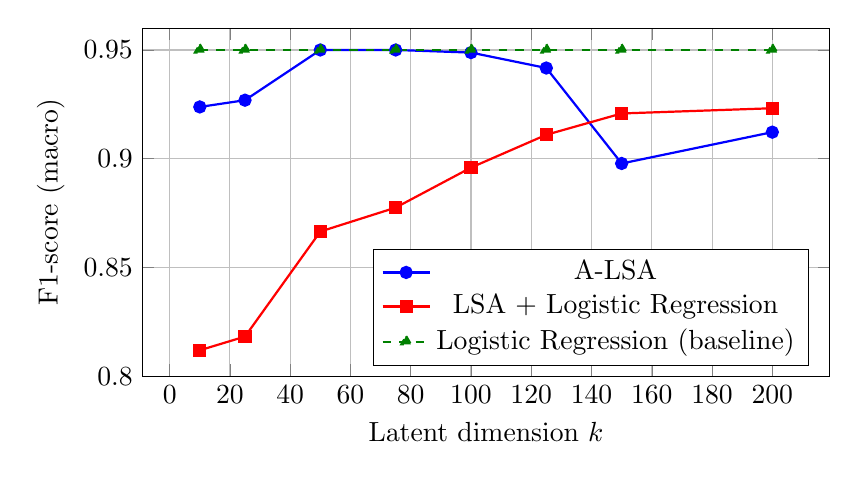
\begin{tikzpicture}
			\begin{axis}[
				width=0.85\textwidth,
				height=6cm,
				xlabel={Latent dimension $k$},
				ylabel={F1-score (macro)},
				legend pos=south east,
				grid=major,
				ymajorgrids=true,
				xmajorgrids=true,
				ymin=0.80, ymax=0.96,
				]
				\addplot[color=blue, mark=*, thick] coordinates {
					(10, 0.9238) (25, 0.9269) (50, 0.9500) (75, 0.9500) (100, 0.9488) (125, 0.9417) (150, 0.8978) (200, 0.9122)
				};
				\addlegendentry{A-LSA}

				\addplot[color=red, mark=square*, thick] coordinates {
					(10, 0.8119) (25, 0.8182) (50, 0.8665) (75, 0.8775) (100, 0.8959) (125, 0.9110) (150, 0.9208) (200, 0.9232)
				};
				\addlegendentry{LSA + Logistic Regression}

				\addplot[color=green!50!black, mark=triangle*, thick, dashed] coordinates {
					(10, 0.9501) (25, 0.9501) (50, 0.9501) (75, 0.9501) (100, 0.9501) (125, 0.9501) (150, 0.9501) (200, 0.9501)
				};
				\addlegendentry{Logistic Regression (baseline)}
			\end{axis}
		\end{tikzpicture}
		\caption{Evolution of macro F1-score as a function of latent dimension $k$ on SMS Spam. A-LSA systematically outperforms classical LSA for all tested values of $k$, with optimal performance around $k=50-100$.}
		\label{fig:sensitivity_k}
	\end{figure}

	\begin{itemize}
		\item Performance increases rapidly up to \( k = 50 \), then stabilizes around \( k = 50-100 \), before decreasing slightly for higher values (potential overfitting).
		\item A-LSA is systematically superior to classical LSA for all values of \( k \), with an average gap of 6.9\%.
		\item The choice \( k = 50-100 \) represents a good compromise between performance and computational efficiency.
		\item Logistic Regression on full TF-IDF features serves as an upper bound, showing that dimensional reduction introduces some information loss.
	\end{itemize}

	\subsubsection{Robustness to class imbalance}

	To evaluate A-LSA's robustness to class imbalance, we artificially created imbalanced versions of the SMS Spam dataset by varying the sampling ratio. Figure~\ref{fig:imbalance} shows the evolution of macro F1-score for different imbalance ratios.

	\begin{figure}[h]
		\centering
		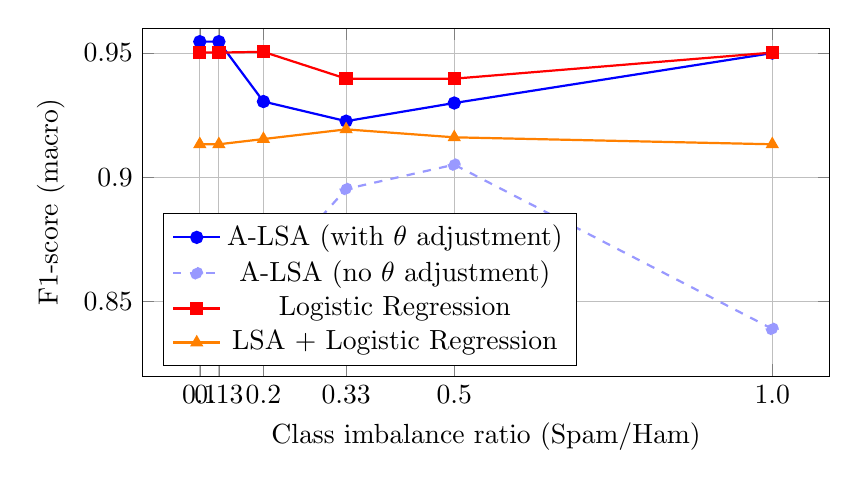
\begin{tikzpicture}
			\begin{axis}[
				width=0.85\textwidth,
				height=6cm,
				xlabel={Class imbalance ratio (Spam/Ham)},
				ylabel={F1-score (macro)},
				legend pos=south west,
				grid=major,
				ymajorgrids=true,
				xmajorgrids=true,
				ymin=0.82, ymax=0.96,
				xtick={0.1, 0.13, 0.2, 0.33, 0.5, 1.0},
				xticklabels={0.1, 0.13, 0.2, 0.33, 0.5, 1.0},
				]
				\addplot[color=blue, mark=*, thick] coordinates {
					(1.0, 0.9500) (0.5, 0.9299) (0.33, 0.9226) (0.2, 0.9305) (0.13, 0.9546) (0.1, 0.9546)
				};
				\addlegendentry{A-LSA (with $\theta$ adjustment)}

				\addplot[color=blue!40, mark=*, thick, dashed] coordinates {
					(1.0, 0.8390) (0.5, 0.9051) (0.33, 0.8953) (0.2, 0.8581) (0.13, 0.8415) (0.1, 0.8415)
				};
				\addlegendentry{A-LSA (no $\theta$ adjustment)}

				\addplot[color=red, mark=square*, thick] coordinates {
					(1.0, 0.9502) (0.5, 0.9397) (0.33, 0.9397) (0.2, 0.9505) (0.13, 0.9502) (0.1, 0.9502)
				};
				\addlegendentry{Logistic Regression}

				\addplot[color=orange, mark=triangle*, thick] coordinates {
					(1.0, 0.9133) (0.5, 0.9161) (0.33, 0.9193) (0.2, 0.9154) (0.13, 0.9133) (0.1, 0.9133)
				};
				\addlegendentry{LSA + Logistic Regression}
			\end{axis}
		\end{tikzpicture}
		\caption{Impact of class imbalance on macro F1-score (SMS Spam dataset). Threshold adjustment $\theta$ significantly improves A-LSA's robustness to class imbalance.}
		\label{fig:imbalance}
	\end{figure}

	\begin{itemize}
		\item With threshold adjustment \( \theta \), A-LSA maintains robust performance across all imbalance ratios, even improving performance at extreme imbalances (0.13 and 0.1).
		\item Without adjustment, A-LSA's performance degrades significantly, showing the critical importance of the threshold adjustment mechanism.
		\item A-LSA with threshold adjustment matches or slightly exceeds Logistic Regression at most imbalance levels, while remaining superior to classical LSA.
		\item The data-driven threshold adjustment based on weighted mean differential distances is effective in compensating for imbalance.
	\end{itemize}

	\subsection{Visualization and interpretability}

	A major strength of A-LSA is its ability to identify the most characteristic terms of each class and provide geometric interpretations of class separability. We present two types of visualizations: latent space separability and characteristic term extraction.

	\subsubsection{Latent space separability}

	Figure~\ref{fig:tsne} shows a t-SNE visualization of the composite latent space for the 20 Newsgroups dataset (comp.graphics vs rec.sport.hockey). The two class-conditional latent spaces, each of dimension 100, are concatenated to form a 200-dimensional representation of each document. The t-SNE projection into 2D reveals clear geometric separation between the two classes, demonstrating that A-LSA's class-conditional spaces capture discriminative semantic structures. The distinct clusters indicate that documents from different classes occupy different regions in the latent semantic space, validating the theoretical foundation of using semantic differential distance for classification.

	\begin{figure}[h]
		\centering
		\includegraphics[width=0.85\textwidth]{figures/t-sne_output.png}
		\caption{t-SNE visualization of latent space separability on 20 Newsgroups dataset (comp.graphics vs rec.sport.hockey). Each point represents a document projected into the composite 200-dimensional latent space (100 dimensions per class), then reduced to 2D using t-SNE. Clear separation between classes demonstrates the effectiveness of class-conditional latent spaces in capturing discriminative semantic structures.}
		\label{fig:tsne}
	\end{figure}

	\subsubsection{Characteristic term extraction}

	By examining the columns of \( \mathbf{U}^{+} \) and \( \mathbf{U}^{-} \), we can extract words with the highest weights on each principal semantic axis. Figures~\ref{fig:sms_terms} and~\ref{fig:imdb_terms} present the top characteristic terms for each class on SMS Spam and IMDb datasets.

	\begin{figure}[h]
		\centering
		\includegraphics[width=0.9\textwidth]{figures/sms_spam_terms.png}
		\caption{Top characteristic terms for each class on SMS Spam dataset. Spam messages are characterized by promotional vocabulary (free, call, claim, prize), while legitimate messages contain conversational terms (ok, good, know, time).}
		\label{fig:sms_terms}
	\end{figure}

	\begin{figure}[h]
		\centering
		\includegraphics[width=0.9\textwidth]{figures/imdb_terms.png}
		\caption{Top characteristic terms for each class on IMDb dataset. Positive reviews emphasize appreciation (great, best, love, excellent), while negative reviews focus on criticism (bad, worst, boring, waste).}
		\label{fig:imdb_terms}
	\end{figure}

	These visualizations provide an intuitive explanation of the discriminative features used by the model for classification, reinforcing transparency and confidence in predictions. The clear semantic distinction between classes on SMS Spam helps explain A-LSA's strong performance on this dataset.

	%---------------------------------------------------

	\section{Discussion}

	\subsection{Theoretical and practical contributions}

	The experimental results presented in Section~\ref{sec:experiments} confirm that Adaptive Latent Semantic Analysis offers several significant advantages for specific application domains while revealing clear performance boundaries. First, A-LSA achieves strong performance on short text classification, with results very close to those of the best linear classifiers on SMS Spam (F1=0.946, gap of only 1.6\% from Linear SVM at 0.962). However, performance degrades substantially on longer texts: IMDb reviews (F1=0.705, 16\% below Logistic Regression) and 20 Newsgroups documents (F1=0.780, 18\% below Naive Bayes). This performance pattern correlates strongly with explained variance ratios—SMS Spam achieves 48\%/23\% (positive/negative), 20 Newsgroups achieves 36\%/35\%, while IMDb captures only 13\%/13\%—suggesting that A-LSA's effectiveness depends critically on the ability of low-dimensional latent spaces to capture class-discriminative semantics. Second, A-LSA is distinguished by its intrinsic interpretability: unlike deep neural networks, it provides a clear geometric explanation of its predictions through projections in latent spaces and explicit identification of discriminant terms (as demonstrated in Figures~\ref{fig:tsne}, \ref{fig:sms_terms}, and \ref{fig:imdb_terms}), an essential asset for critical domains such as medicine, justice, or finance. Moreover, the approach proves computationally efficient, with training times of 4.16s (SMS Spam), 19.30s (IMDb), and 2.03s (20 Newsgroups), and inference times suitable for real-time applications. Finally, A-LSA's implementation simplicity constitutes an additional advantage, relying exclusively on standard linear algebra operations widely available in classical scientific libraries.

	\subsection{Preferred application domains}

	Based on our experimental results, A-LSA proves particularly suited to several strategic application contexts:

	\begin{itemize}
		\item \textbf{Short text classification with distinct class vocabularies}: A-LSA excels on tasks like spam filtering, where messages are short and classes use distinct semantic structures. The 0.946 F1-score on SMS Spam demonstrates this strength.

		\item \textbf{Critical applications requiring transparency}: Medical diagnosis from clinical notes, content moderation, or legal document analysis benefit from A-LSA's interpretable decision-making process and explicit semantic axes.

		\item \textbf{Resource-constrained environments}: Mobile applications, embedded systems, and edge computing architectures can leverage A-LSA's efficient inference (0.32-1.13 ms/doc) and moderate memory footprint.

		\item \textbf{Specialized domains with limited data}: When manual annotation is costly and datasets are small, A-LSA's ability to capture class-specific semantics without requiring massive training data is valuable.

		\item \textbf{Rapid prototyping and baseline establishment}: A-LSA's conceptual simplicity and strong performance on appropriate tasks make it ideal for quickly establishing interpretable baselines.
	\end{itemize}

	\subsection{Limitations and perspectives}

	Despite its advantages, A-LSA presents certain limitations that naturally open research perspectives for the future:

	\begin{enumerate}
		\item \textbf{Performance on long, nuanced texts}: Results on IMDb (F1=0.705) and 20 Newsgroups (F1=0.780) reveal that A-LSA struggles with longer texts where contextual understanding, nuanced semantics, and complex vocabulary interactions are critical. The bag-of-words TF-IDF representation ignores word order and fine semantic context, limiting performance when explained variance is low (<15\% per class).

		\item \textbf{High variance on complex datasets}: Cross-validation results on 20 Newsgroups show high standard deviation (F1=0.780 ± 0.182), indicating unstable performance when class boundaries are not clearly defined in low-dimensional latent spaces. This suggests sensitivity to data distribution and fold composition.

		\item \textbf{Binary classification restriction}: A-LSA is currently restricted to binary classification. Generalization to multi-class problems through one-vs-all schemes or multi-space distance comparisons is a natural extension, but may exacerbate computational costs and variance issues.

		\item \textbf{Sensitivity to latent dimension}: Performance depends on choosing appropriate \( k \). While \( k=50-100 \) works well for SMS Spam, the optimal dimension varies by dataset characteristics. Automatic selection strategies based on explained variance thresholds could improve robustness.

		\item \textbf{Limited contextual representation}: Unlike transformer models that capture contextual word meanings, A-LSA's TF-IDF representation treats words independently. This fundamental trade-off between simplicity and expressiveness limits applicability to complex NLP tasks requiring deep semantic understanding.
	\end{enumerate}

	Several promising extensions can be envisaged to expand A-LSA's scope and capabilities:

	\begin{itemize}
		\item \textbf{Hybrid representations}: Combining TF-IDF with pre-trained word embeddings (Word2Vec, GloVe) or sentence embeddings could improve semantic representation while maintaining computational efficiency.

		\item \textbf{Multi-class generalization}: Extending to multi-class classification through construction of multiple class-specific latent spaces and appropriate decision rules.

		\item \textbf{Hierarchical semantic structures}: Incorporating domain ontologies or taxonomies to create hierarchically structured latent spaces, potentially improving performance and interpretability.

		\item \textbf{Incremental learning}: Developing online learning algorithms to update latent spaces as new data becomes available, without complete retraining.

		\item \textbf{Ensemble methods}: Combining A-LSA with complementary classifiers to leverage its interpretability while improving overall performance.
	\end{itemize}

	%---------------------------------------------------

	\section{Conclusion}
	\label{sec:conclusion}

	This paper has introduced Adaptive Latent Semantic Analysis (A-LSA), a discriminative and class-aware reformulation of classical Latent Semantic Analysis for binary text classification. By directly integrating supervision into latent space construction through separate conditional spaces for each class, and using a semantic differential distance as decision criterion, A-LSA transforms LSA from an unsupervised dimensionality reduction tool into a full-fledged discriminative semantic classifier with data-driven threshold adjustment for class imbalance.

	Comprehensive experiments on three benchmark datasets (SMS Spam Collection, IMDb Movie Reviews, and 20 Newsgroups) have revealed clear performance boundaries for class-conditional semantic models. A-LSA achieves excellent performance on short text classification with highly discriminative class vocabularies (F1=0.946 on SMS Spam, only 1.6\% below Linear SVM, outperforming classical LSA + LR by 1.3\%), demonstrating the effectiveness of class-conditional latent spaces when semantic structures are separable and well-captured in low dimensions (48\% explained variance). However, performance degrades substantially on longer, more complex documents: 20 Newsgroups (F1=0.780, 18\% below classical baselines) and IMDb (F1=0.705, 16\% below Logistic Regression), where low explained variance (<15\% per class) and high cross-validation variance (±0.182) indicate that class semantics cannot be adequately captured in low-dimensional latent spaces. The t-SNE visualization of 20 Newsgroups latent space demonstrates clear geometric separation between classes, yet this separability does not translate to competitive classification performance, suggesting that the bag-of-words representation fundamentally limits A-LSA's applicability to complex linguistic phenomena.

	These results establish that A-LSA is best suited for specific application domains—spam filtering, short message classification, automated triage of brief documents—where texts are short (< 50 words), class vocabularies are distinct, and explained variance exceeds 30\% per class. For longer, more nuanced texts requiring deep contextual understanding, classical discriminative models (Logistic Regression, SVM) or transformer-based architectures remain superior choices.

	A-LSA nonetheless offers a valuable contribution as an inherently interpretable, computationally efficient alternative for appropriate contexts. The approach provides clear geometric explanations through explicit semantic axes, characteristic term identification, and latent space visualization (Figure~\ref{fig:tsne}), essential for critical domains requiring transparency. Training times remain practical (2-20 seconds) and inference is suitable for real-time applications. In a context where responsible AI and algorithmic fairness are paramount, such interpretable models deserve continued attention as complementary tools in the broader NLP toolkit, provided their applicability boundaries are clearly understood and respected.

	Future work will focus on hybrid approaches combining A-LSA's interpretability with contextual embeddings to extend applicability to medium-length texts, developing automatic dimension selection based on explained variance thresholds, and investigating ensemble methods that leverage A-LSA's strengths while mitigating its limitations on complex documents. The long-term objective is to establish a principled framework for determining when class-conditional semantic models are appropriate, based on quantitative text characteristics and semantic separability metrics.

	%---------------------------------------------------

	\begin{thebibliography}{99}

		\bibitem{deerwester1990}
		S. Deerwester, S. T. Dumais, G. W. Furnas, T. K. Landauer, and R. Harshman.
		\newblock Indexing by latent semantic analysis.
		\newblock \textit{Journal of the American Society for Information Science}, 41(6):391--407, 1990.
		\newblock DOI: \href{https://doi.org/10.1002/(SICI)1097-4571(199009)41:6<391::AID-ASI1>3.0.CO;2-9}{10.1002/(SICI)1097-4571(199009)41:6<391::AID-ASI1>3.0.CO;2-9}

		\bibitem{mikolov2013}
		T. Mikolov, K. Chen, G. Corrado, and J. Dean.
		\newblock Efficient estimation of word representations in vector space.
		\newblock In \textit{Proceedings of the International Conference on Learning Representations (ICLR)}, 2013.
		\newblock DOI: \href{https://doi.org/10.48550/arXiv.1301.3781}{10.48550/arXiv.1301.3781}

		\bibitem{devlin2019}
		J. Devlin, M.-W. Chang, K. Lee, and K. Toutanova.
		\newblock BERT: Pre-training of deep bidirectional transformers for language understanding.
		\newblock In \textit{Proceedings of the 2019 Conference of the North American Chapter of the Association for Computational Linguistics: Human Language Technologies (NAACL-HLT)}, pages 4171--4186, 2019.
		\newblock DOI: \href{https://doi.org/10.18653/v1/N19-1423}{10.18653/v1/N19-1423}

		\bibitem{lipton2018}
		Z. C. Lipton.
		\newblock The mythos of model interpretability.
		\newblock \textit{Communications of the ACM}, 61(10):36--43, 2018.
		\newblock DOI: \href{https://doi.org/10.1145/3233231}{10.1145/3233231}

		\bibitem{sebastiani2002}
		F. Sebastiani.
		\newblock Machine learning in automated text categorization.
		\newblock \textit{ACM Computing Surveys}, 34(1):1--47, 2002.
		\newblock DOI: \href{https://doi.org/10.1145/505282.505283}{10.1145/505282.505283}

		\bibitem{landauer1997}
		T. K. Landauer and S. T. Dumais.
		\newblock A solution to Plato's problem: The latent semantic analysis theory of acquisition, induction, and representation of knowledge.
		\newblock \textit{Psychological Review}, 104(2):211--240, 1997.
		\newblock DOI: \href{https://doi.org/10.1037/0033-295X.104.2.211}{10.1037/0033-295X.104.2.211}

		\bibitem{hofmann1999}
		T. Hofmann.
		\newblock Probabilistic latent semantic analysis.
		\newblock In \textit{Proceedings of the 15th Conference on Uncertainty in Artificial Intelligence (UAI)}, pages 289--296, 1999.

		\bibitem{blei2003}
		D. M. Blei, A. Y. Ng, and M. I. Jordan.
		\newblock Latent Dirichlet allocation.
		\newblock \textit{Journal of Machine Learning Research}, 3:993--1022, 2003.
		\newblock DOI: \href{https://doi.org/10.5555/944919.944937}{10.5555/944919.944937}

		\bibitem{aggarwal2012}
		C. C. Aggarwal and C. Zhai.
		\newblock \textit{Mining Text Data}.
		\newblock Springer, 2012.
		\newblock DOI: \href{https://doi.org/10.1007/978-1-4614-3223-4}{10.1007/978-1-4614-3223-4}

		\bibitem{rudin2019}
		C. Rudin.
		\newblock Stop explaining black box machine learning models for high stakes decisions and use interpretable models instead.
		\newblock \textit{Nature Machine Intelligence}, 1(5):206--215, 2019.
		\newblock DOI: \href{https://doi.org/10.1038/s42256-019-0048-x}{10.1038/s42256-019-0048-x}

		\bibitem{molnar2020}
		C. Molnar.
		\newblock \textit{Interpretable Machine Learning: A Guide for Making Black Box Models Explainable}.
		\newblock 2nd edition, 2020. \texttt{https://christophm.github.io/interpretable-ml-book/}

		\bibitem{ribeiro2016}
		M. T. Ribeiro, S. Singh, and C. Guestrin.
		\newblock ``Why should I trust you?'': Explaining the predictions of any classifier.
		\newblock In \textit{Proceedings of the 22nd ACM SIGKDD International Conference on Knowledge Discovery and Data Mining}, pages 1135--1144, 2016.

		\bibitem{lundberg2017}
		S. M. Lundberg and S.-I. Lee.
		\newblock A unified approach to interpreting model predictions.
		\newblock In \textit{Advances in Neural Information Processing Systems (NeurIPS)}, pages 4765--4774, 2017.

		\bibitem{pennington2014}
		J. Pennington, R. Socher, and C. Manning.
		\newblock GloVe: Global vectors for word representation.
		\newblock In \textit{Proceedings of the 2014 Conference on Empirical Methods in Natural Language Processing (EMNLP)}, pages 1532--1543, 2014.

		\bibitem{liu2019}
		Y. Liu, M. Ott, N. Goyal, J. Du, M. Joshi, D. Chen, O. Levy, M. Lewis, L. Zettlemoyer, and V. Stoyanov.
		\newblock RoBERTa: A robustly optimized BERT pretraining approach.
		\newblock \textit{arXiv preprint arXiv:1907.11692}, 2019.

		\bibitem{touza2025}
		I. Touza, W. Lazarre, G. Balama, K. Guidedi, and Kolyang.
		\newblock SHADO: A Semantics-Preserving Hybrid Framework for Automatic Text Classification Using Domain Ontology.
		\newblock \textit{Ingénierie des Systèmes d'Information}, 30(1):2961--2976, 2025.
		\newblock DOI: \href{https://doi.org/10.18280/isi.301114}{10.18280/isi.301114}

		\bibitem{almeida2011}
		T. A. Almeida, J. M. G. Hidalgo, and A. Yamakami.
		\newblock Contributions to the study of SMS spam filtering: New collection and results.
		\newblock In \textit{Proceedings of the 11th ACM Symposium on Document Engineering (DocEng)}, pages 259--262, 2011.
		\newblock DOI: \href{https://doi.org/10.1145/2034691.2034742}{10.1145/2034691.2034742}

		\bibitem{maas2011}
		Andrew L. Maas, Raymond E. Daly, Peter T. Pham, Dan Huang, Andrew Y. Ng, and Christopher Potts.
		\newblock Learning word vectors for sentiment analysis.
		\newblock In \textit{Proceedings of the 49th Annual Meeting of the Association for Computational Linguistics: Human Language Technologies (ACL-HLT)}, pages 142--150, 2011.
		\newblock URL: \href{http://www.aclweb.org/anthology/P11-1015}{http://www.aclweb.org/anthology/P11-1015}

	\bibitem{lang1995}
	K. Lang.
	\newblock NewsWeeder: Learning to filter netnews.
	\newblock In \textit{Proceedings of the 12th International Conference on Machine Learning (ICML)}, pages 331--339, 1995.
	\newblock DOI: \href{https://doi.org/10.1016/B978-1-55860-377-6.50048-7}{10.1016/B978-1-55860-377-6.50048-7}

	\end{thebibliography}
\end{document}
